\section{Исследование ИС ADG408 или ADG508 в качестве
коммутатора MUX 8 – 1 цифровых сигналов}

($D_0 \dots D_7$ : 01001000)

Ниже, на рисунке \ref{1}, расположена исследовательская установка. На рисунке \ref{2} результаты работы логического анализатора.

\begin{figure}[ht]
    \centering
    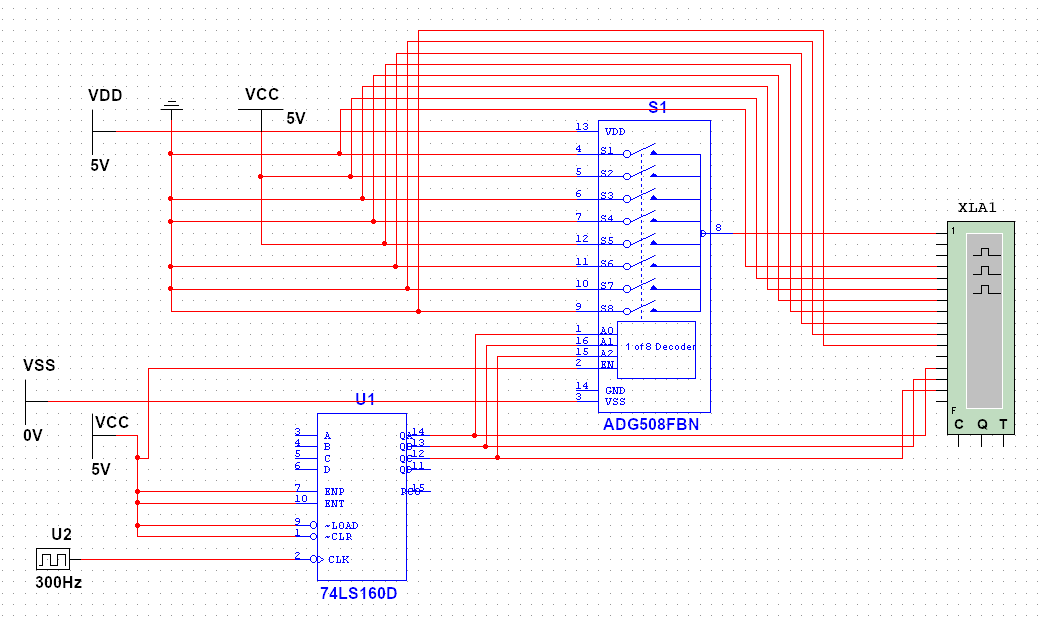
\includegraphics[width=\linewidth]{img/1.png}
    \caption{Схема исследования ИС ADG508.}
    \label{1}
\end{figure}

\begin{figure}[ht]
    \centering
    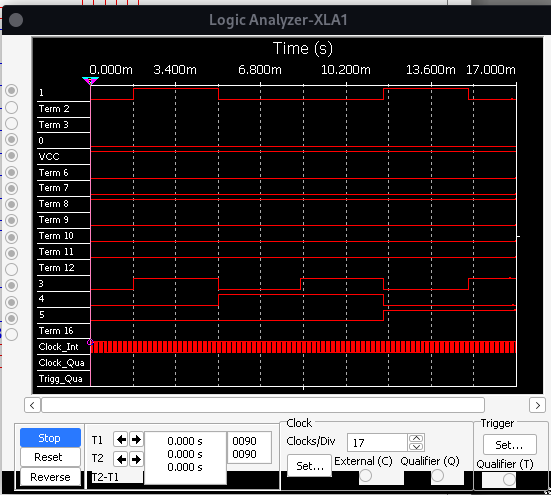
\includegraphics[width=\linewidth]{img/2.png}
    \caption{Временные диаграммы ИС ADG508.}
    \label{2}
\end{figure}

Мультиплексор может быть коммутатором цифровых сигналов. Изучив сигналы, приходим к выводу что они совпадают с входными данными.

\clearpage

\section{Исследование ИС ADG408 или ADG508 в качестве
коммутатора MUX 8 – 1 аналоговых сигналов}

\begin{figure}[ht]
    \centering
    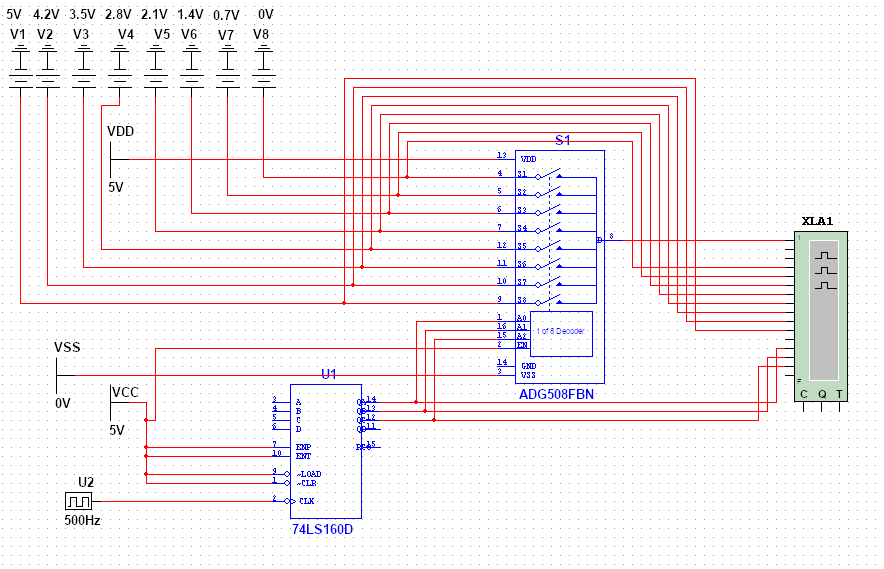
\includegraphics[width=\linewidth]{img/3.png}
    \caption{Схема исследования ИС ADG508 в качестве коммутатора аналоговых сигналов.}
    \label{3}
\end{figure}

На мультиплексоре получается получаем истину при достижении напряжения больше чем половина напряжения $EN$ (рисунок \ref{4}).

\begin{figure}[ht]
    \centering
    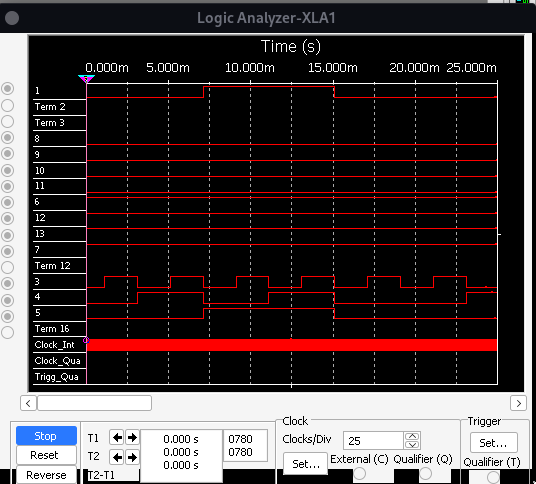
\includegraphics[width=\linewidth]{img/4.png}
    \caption{Схема исследования ИС ADG508 в качестве коммутатора аналоговых сигналов.}
    \label{4}
\end{figure}

\clearpage

\section{Исследование ИС ADG408 или ADG508 как
коммутатора MUX 8 – 1 цифровых сигналов в качестве
формирователя ФАЛ четырех переменных}

($D_{0}...D_{7}$: 01110011)

\begin{figure}[ht]
    \centering
    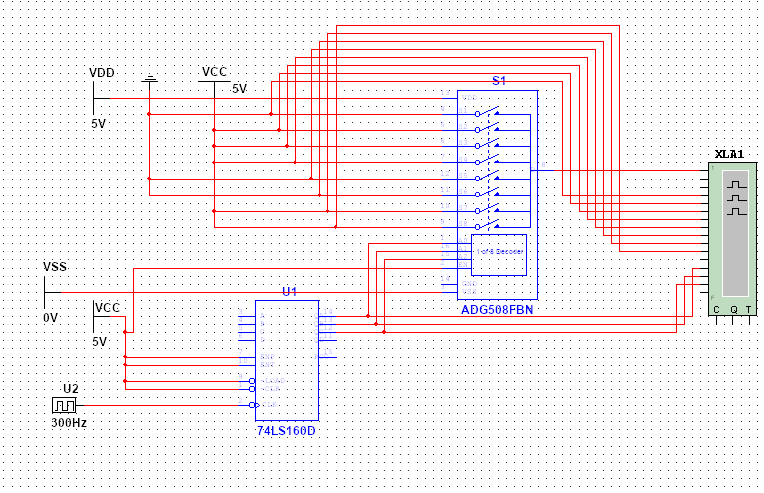
\includegraphics[width=\linewidth]{img/5.png}
    \caption{Схема исследования ИС ADG508 в качестве формирователя ФАЛ четырех переменных.}
    \label{5}
\end{figure}

\begin{figure}[ht]
    \centering
    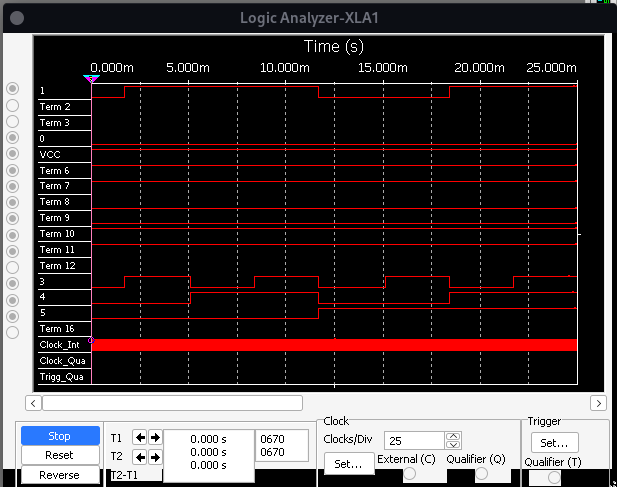
\includegraphics[width=\linewidth]{img/6.png}
    \caption{Временные диаграммы ИС ADG508 в качестве формирователя ФАЛ четырех переменных.}
    \label{6}
\end{figure}

\clearpage

\section{Наращивание мультиплексора}

($D_{0}...D_{15}$: 0001 0000 0001 0000)

Ниже на рисунке \ref{7} представлена схема реализующая заданную функцию с помощью четырех мультиплексоров 8-1 и дешифратора 2-4.

\begin{figure}[ht]
    \centering
    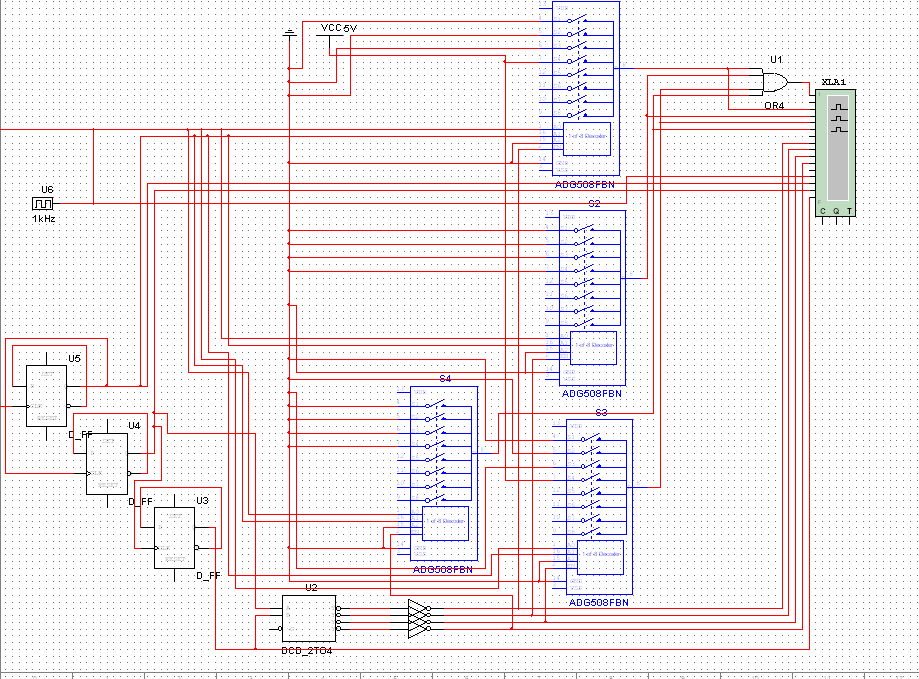
\includegraphics[width=\linewidth]{img/7.png}
    \caption{Схема наращивания мкльтиплексора.}
    \label{7}
\end{figure}

\begin{figure}[ht]
    \centering
    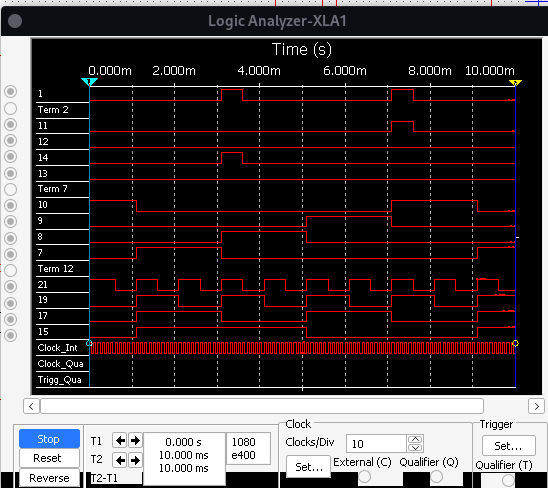
\includegraphics[width=\linewidth]{img/8.png}
    \caption{Временная диаграмма полученной схемы.}
    \label{8}
\end{figure}

Как видно на диаграмме на рисунке \ref{8}, значения на выходе повторяют заданный набор значений. Из чего можно сделать вывод о том, что схема работает правильно.
